\documentclass[aspectratio=169,10pt]{beamer}

\usepackage[T1]{fontenc}
\usepackage{lmodern}
\usepackage{microtype}
\usepackage{amsmath,amssymb}
\usepackage{booktabs}
\usepackage{tabularx}
\usepackage{array}
\usepackage{tikz}
\usepackage{pgfpages}
\usetikzlibrary{arrows.meta,positioning,calc,fit}

\definecolor{Ink}{HTML}{17252C}
\definecolor{Slate}{HTML}{475A63}
\definecolor{Muted}{HTML}{738188}
\definecolor{Rule}{HTML}{D7DEDF}
\definecolor{Panel}{HTML}{F3F6F6}
\definecolor{Accent}{HTML}{0B7781}
\definecolor{AccentSoft}{HTML}{E6F2F2}
\definecolor{Amber}{HTML}{A66A12}
\definecolor{AmberSoft}{HTML}{F8F0E3}
\definecolor{Fault}{HTML}{A7433B}
\definecolor{FaultSoft}{HTML}{F8ECEA}

\setbeamertemplate{navigation symbols}{}
\setbeamercolor{normal text}{fg=Ink,bg=white}
\setbeamercolor{frametitle}{fg=Ink,bg=white}
\setbeamercolor{title}{fg=Ink}
\setbeamercolor{subtitle}{fg=Slate}
\setbeamerfont{title}{series=\bfseries,size=\fontsize{25}{29}}
\setbeamerfont{subtitle}{size=\fontsize{12}{15}}
\setbeamerfont{frametitle}{series=\bfseries,size=\fontsize{16.5}{20}}
\setbeamerfont{footline}{size=\fontsize{7.5}{9}}
\setbeamersize{text margin left=0.62cm,text margin right=0.62cm}
\setbeamertemplate{itemize item}{\color{Accent}\raisebox{0.15ex}{\scriptsize$\blacksquare$}}
\setbeamertemplate{itemize subitem}{\color{Muted}\raisebox{0.15ex}{\tiny$\blacksquare$}}
\setlength{\leftmargini}{1.2em}
\setlength{\leftmarginii}{1.1em}

\setbeamertemplate{frametitle}{%
  \vspace{0.16cm}%
  \insertframetitle\par
  \vspace{0.08cm}%
  {\color{Rule}\rule{\textwidth}{0.45pt}}%
}

\setbeamertemplate{footline}{%
  \leavevmode%
  \hbox{%
    \begin{beamercolorbox}[wd=.82\paperwidth,ht=2.6ex,dp=1.1ex,leftskip=.62cm]{normal text}%
      \color{Muted}UNO / V2 atomic storage
    \end{beamercolorbox}%
    \begin{beamercolorbox}[wd=.18\paperwidth,ht=2.6ex,dp=1.1ex,rightskip=.62cm plus1fil]{normal text}%
      \hfill\color{Muted}\insertframenumber
    \end{beamercolorbox}%
  }%
}

\ifdefined\shownotes
  \setbeameroption{show notes on second screen=right}
\else
  \setbeameroption{hide notes}
\fi

\newcommand{\eyebrow}[1]{\textcolor{Accent}{\bfseries\scriptsize\MakeUppercase{#1}}}
\newcommand{\muted}[1]{\textcolor{Muted}{#1}}
\newcommand{\cost}[1]{\textcolor{Fault}{#1}}
\newcommand{\takeaway}[1]{%
  \begin{beamercolorbox}[wd=\dimexpr\textwidth-0.36cm\relax,sep=0.18cm,leftskip=0.08cm,rightskip=0.08cm]{takeaway}%
    \color{Ink}\small #1
  \end{beamercolorbox}%
}
\setbeamercolor{takeaway}{fg=Ink,bg=AccentSoft}

\tikzset{
  box/.style={draw=Rule,fill=white,line width=.55pt,minimum height=.72cm,align=center,inner xsep=.14cm,inner ysep=.1cm},
  panel/.style={draw=Rule,fill=Panel,line width=.55pt,align=left,inner sep=.18cm},
  root/.style={draw=Accent,fill=AccentSoft,line width=.7pt,minimum height=.68cm,align=center,inner xsep=.16cm},
  oldroot/.style={draw=Muted,fill=Panel,line width=.6pt,minimum height=.68cm,align=center,inner xsep=.16cm},
  warn/.style={draw=Amber,fill=AmberSoft,line width=.6pt,align=center,inner sep=.16cm},
  bad/.style={draw=Fault,fill=FaultSoft,line width=.6pt,align=center,inner sep=.16cm},
  flow/.style={-{Latex[length=2.2mm,width=1.35mm]},draw=Accent,line width=.8pt},
  plainline/.style={draw=Slate,line width=.65pt},
  faintline/.style={draw=Rule,line width=.55pt}
}

\title{Crash-atomic append publication,\\built on ordinary blobs}
\subtitle{Participant-linked UNO / V2 with write-once payload and checked pages}
\author{Commonware storage design walkthrough}
\date{PR \#4368}

\begin{document}

\begin{frame}[plain]
  \vspace{0.95cm}
  \eyebrow{Commonware storage}

  \vspace{0.28cm}
  {\usebeamerfont{title}\color{Ink}\inserttitle\par}

  \vspace{0.28cm}
  {\usebeamerfont{subtitle}\color{Slate}\insertsubtitle\par}

  \vspace{0.18cm}
  {\small\color{Amber}\textbf{Status: opt-in ALPHA API; ordinary Storage and V0/V1 remain unchanged.}\par}

  \vfill
  \begin{center}
    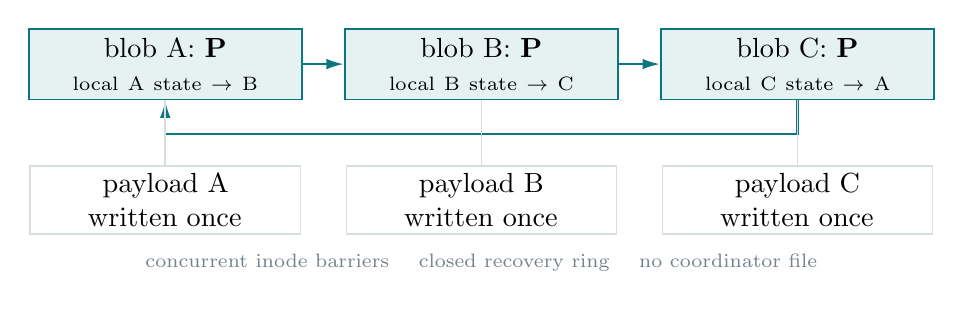
\begin{tikzpicture}[node distance=.52cm]
      \node[root,text width=3.15cm,minimum height=.9cm] (a) {blob A: \textbf{P}\\\scriptsize local A state $\rightarrow$ B};
      \node[root,text width=3.15cm,minimum height=.9cm,right=of a] (b) {blob B: \textbf{P}\\\scriptsize local B state $\rightarrow$ C};
      \node[root,text width=3.15cm,minimum height=.9cm,right=of b] (c) {blob C: \textbf{P}\\\scriptsize local C state $\rightarrow$ A};
      \draw[flow] (a) -- (b);
      \draw[flow] (b) -- (c);
      \draw[flow] (c.south) -- ++(0,-.43cm) -| (a.south);

      \node[box,text width=3.15cm,minimum height=.46cm,below=.82cm of a] (pa) {payload A written once};
      \node[box,text width=3.15cm,minimum height=.46cm,below=.82cm of b] (pb) {payload B written once};
      \node[box,text width=3.15cm,minimum height=.46cm,below=.82cm of c] (pc) {payload C written once};
      \draw[faintline] (a) -- (pa);
      \draw[faintline] (b) -- (pb);
      \draw[faintline] (c) -- (pc);
      \node[below=.12cm of pb,font=\scriptsize,text=Muted] {concurrent inode barriers \quad closed recovery ring \quad no coordinator file};
    \end{tikzpicture}
  \end{center}

  \vfill
  {\color{Muted}\small\insertauthor\hfill\insertdate}

  \note{The goal is not a general transactional filesystem. It is the narrower primitive our journals actually need: append, rewind, and delete, with publication at the existing sync boundary. AtomicStorage, AtomicBlob, BatchStorage, BatchOperation, and the atomic paged-buffer helpers are explicitly ALPHA; the ordinary BETA storage surface remains unchanged. UNO is the development nickname for the one-write, one-hot-path-barrier target. Each participant carries only its local proof and an exact link to the next participant; no payload or complete group descriptor is replicated.}
\end{frame}

\begin{frame}[t]{The contract we actually need}
  \vspace{0.02cm}
  \begin{columns}[T,onlytextwidth]
    \begin{column}{0.49\textwidth}
      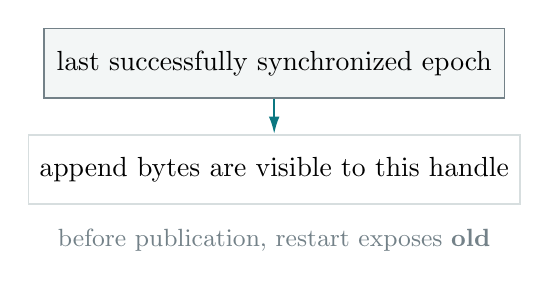
\begin{tikzpicture}[node distance=.45cm]
        \node[oldroot,minimum width=5.7cm,minimum height=.88cm] (old) {last successfully synchronized epoch};
        \node[box,minimum width=5.7cm,below=of old,minimum height=.88cm] (pending) {append bytes are visible to this handle};
        \draw[flow] (old) -- (pending);
        \node[below=.18cm of pending,font=\small,text=Muted,align=center] {before publication, restart exposes \textbf{old}};
      \end{tikzpicture}
    \end{column}
    \begin{column}{0.49\textwidth}
      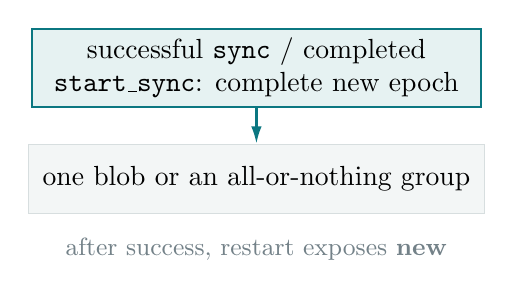
\begin{tikzpicture}[node distance=.45cm]
        \node[root,minimum width=5.7cm,minimum height=.88cm] (new) {successful \texttt{sync} / completed\\\texttt{start\_sync}: complete new epoch};
        \node[panel,minimum width=5.7cm,below=of new,minimum height=.88cm,align=center] (group) {one blob or an all-or-nothing group};
        \draw[flow] (new) -- (group);
        \node[below=.18cm of group,font=\small,text=Muted,align=center] {after success, restart exposes \textbf{new}};
      \end{tikzpicture}
    \end{column}
  \end{columns}

  \vspace{0.38cm}
  \begin{columns}[T,onlytextwidth]
    \begin{column}{0.32\textwidth}
      \eyebrow{Fault model}\par\smallskip
      \small Any subset of writes not covered by a completed durability barrier may survive.
    \end{column}
    \begin{column}{0.32\textwidth}
      \eyebrow{Indeterminate window}\par\smallskip
      \small A failed or cancelled sync may recover old or complete new---never a mixture.
    \end{column}
    \begin{column}{0.32\textwidth}
      \eyebrow{Performance target}\par\smallskip
      \small Keep ordinary append behavior: write payload once and pay at the existing sync.
    \end{column}
  \end{columns}

  \vfill
  \takeaway{Atomicity is a crash-recovery property; durability remains attached to \texttt{sync} or completion of \texttt{start\_sync}.}

  \note{This distinction is important. Appending does not promise durability. A successful sync does; start_sync starts the self-driving durability operation and its completion handle reports the result. If publication is interrupted after I/O starts, its result is indeterminate in the usual storage sense, but recovery must still choose one complete epoch. The tests use the stronger arbitrary-subset model, not a prefix-of-writes assumption.}
\end{frame}

\begin{frame}[t]{Before: each journal coordinated its own crash state}
  \vspace{0.03cm}
  \begin{columns}[T,onlytextwidth]
    \begin{column}{0.49\textwidth}
      \eyebrow{Legacy fixed journal}

      \vspace{0.18cm}
      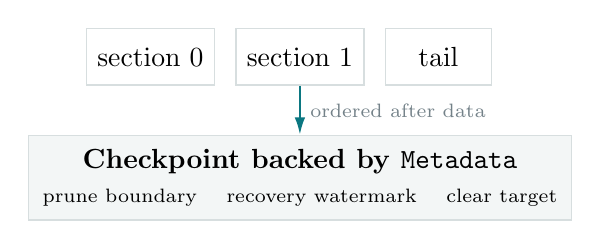
\begin{tikzpicture}[node distance=.25cm]
        \node[box,minimum width=1.35cm] (f0) {section 0};
        \node[box,minimum width=1.35cm,right=of f0] (f1) {section 1};
        \node[box,minimum width=1.35cm,right=of f1] (f2) {tail};
        \node[panel,minimum width=5.8cm,below=.62cm of f1,align=center] (meta) {\textbf{Checkpoint backed by \texttt{Metadata}}\\\scriptsize prune boundary \quad recovery watermark \quad clear target};
        \draw[flow] (f1.south) -- node[right,font=\scriptsize,text=Muted]{ordered after data} (meta.north);
      \end{tikzpicture}
    \end{column}
    \begin{column}{0.49\textwidth}
      \eyebrow{Legacy variable journal}

      \vspace{0.18cm}
      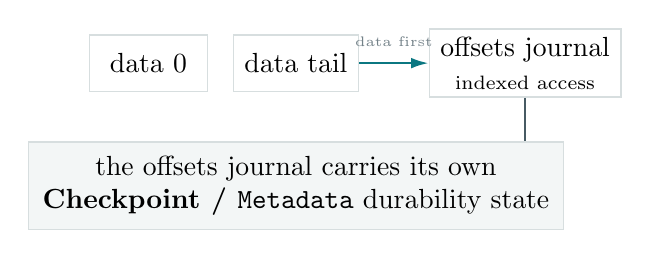
\begin{tikzpicture}[node distance=.31cm]
        \node[box,minimum width=1.5cm] (d0) {data 0};
        \node[box,minimum width=1.5cm,right=of d0] (d1) {data tail};
        \node[box,minimum width=2.15cm,right=.88cm of d1] (idx) {offsets journal\\\scriptsize indexed access};
        \draw[flow] (d1) -- node[above=.08cm,font=\tiny,text=Muted]{data first} (idx);
        \node[panel,minimum width=5.8cm,below=.62cm of d1,align=center] (vmeta) {the offsets journal carries its own\\\textbf{Checkpoint / \texttt{Metadata}} durability state};
        \draw[plainline] (idx.south) -- (idx.south |- vmeta.north);
      \end{tikzpicture}
    \end{column}
  \end{columns}

  \vspace{0.24cm}
  \small
  \begin{itemize}\setlength\itemsep{0.08cm}
    \item \texttt{commit}, \texttt{start\_sync}, and stronger \texttt{sync} kept data, indexes, and recovery hints in a safe order.
    \item The storage API had no primitive for atomically publishing several blob roots together.
  \end{itemize}

  \vfill
  \takeaway{The journals were correct, but every compound structure owned a bespoke durability protocol.}

  \note{Be precise about terminology here. The variable offsets journal is a real index and remains useful. The removable object is the separate Metadata-backed checkpoint used for boundary, watermark, and clear intent. Legacy sync semantics grew around maintaining the ordering between those pieces.}
\end{frame}

\begin{frame}[t]{The append-only boundary makes rollback cheap}
  \vspace{0cm}
  \eyebrow{A general transaction engine would need rollback material}

  \vspace{0.04cm}
  \begin{columns}[T,onlytextwidth]
    \begin{column}{0.32\textwidth}
      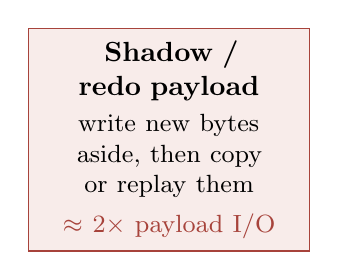
\begin{tikzpicture}
        \node[bad,text width=3.25cm,minimum height=1.7cm] {\textbf{Shadow / redo payload}\\[.08cm]\small write new bytes aside, then copy or replay them\\[.08cm]\cost{$\approx 2\times$ payload I/O}};
      \end{tikzpicture}
    \end{column}
    \begin{column}{0.32\textwidth}
      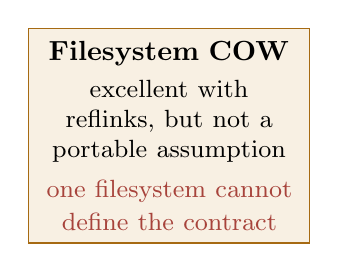
\begin{tikzpicture}
        \node[warn,text width=3.25cm,minimum height=1.7cm] {\textbf{Filesystem COW}\\[.08cm]\small excellent with reflinks, but not a portable assumption\\[.08cm]\cost{one filesystem cannot define the contract}};
      \end{tikzpicture}
    \end{column}
    \begin{column}{0.32\textwidth}
      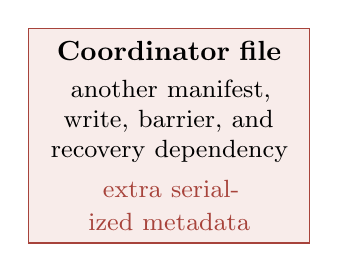
\begin{tikzpicture}
        \node[bad,text width=3.25cm,minimum height=1.7cm] {\textbf{Coordinator file}\\[.08cm]\small another manifest, write, barrier, and recovery dependency\\[.08cm]\cost{extra serialized metadata}};
      \end{tikzpicture}
    \end{column}
  \end{columns}

  \vspace{0.12cm}
  \begin{center}
    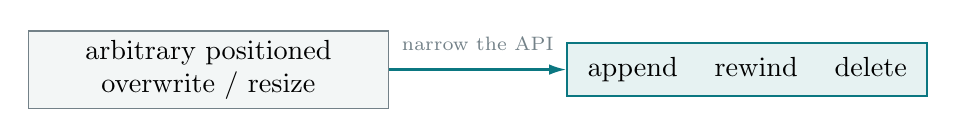
\begin{tikzpicture}
      \node[oldroot,text width=4.25cm] (general) {arbitrary positioned overwrite / resize};
      \node[root,text width=4.25cm,right=2.25cm of general] (narrow) {append \quad rewind \quad delete};
      \draw[flow] (general) -- (narrow);
      \node[above=.12cm of $(general.east)!0.5!(narrow.west)$,font=\scriptsize,text=Muted] {narrow the API};
    \end{tikzpicture}
  \end{center}

  \vspace{0.04cm}
  \small A checksum can detect a torn overwrite; it cannot restore overwritten bytes. Append-only preserves the old prefix, so a root can select a complete visible prefix.

  \vfill
  \takeaway{The decisive optimization is an API constraint: preserve old bytes and publish a new length.}

  \note{CRC32C is useful once the primitive preserves the old prefix, but it is not itself rollback material. It is not an authentication mechanism and it does not protect against someone deliberately editing the disk and checksum. The threat here is crash-torn local storage. For random overwrite, a CRC only tells us that data is bad; it does not restore the overwritten bytes.}
\end{frame}

\begin{frame}[t]{Architecture: UNO wraps an ordinary \texttt{Blob}}
  \vspace{-0.07cm}
  \begin{center}
    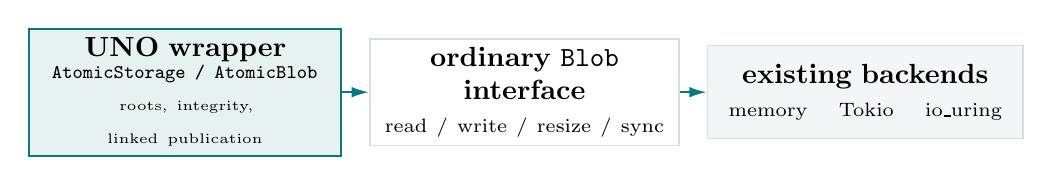
\begin{tikzpicture}[node distance=.34cm]
      \node[root,text width=3.65cm,minimum height=1.18cm] (api) {\textbf{UNO wrapper}\\\scriptsize \texttt{AtomicStorage / AtomicBlob}\\[-.02cm]\tiny roots, integrity, linked publication};
      \node[box,text width=3.65cm,minimum height=1.18cm,right=of api] (blob) {\textbf{ordinary \texttt{Blob} interface}\\\scriptsize read / write / resize / sync};
      \node[panel,text width=3.65cm,minimum height=1.18cm,right=of blob,align=center] (backend) {\textbf{existing backends}\\\scriptsize memory \quad Tokio \quad io\_uring};
      \draw[flow] (api) -- (blob);
      \draw[flow] (blob) -- (backend);
    \end{tikzpicture}
  \end{center}

  \vspace{0.03cm}
  \eyebrow{The wrapper's backing-blob coordinates}

  \vspace{0.01cm}
  \begin{center}
    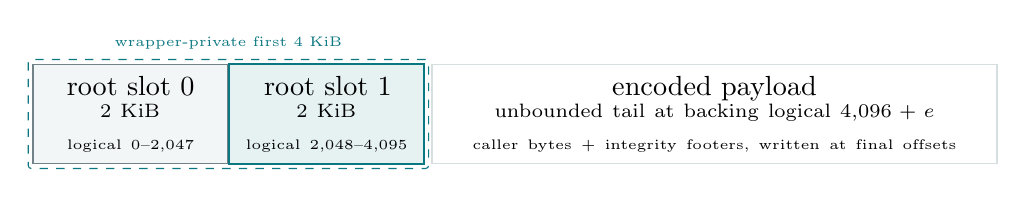
\begin{tikzpicture}[node distance=0cm]
      \node[oldroot,text width=2.15cm,minimum height=1.26cm] (r0) {root slot 0\\\scriptsize 2 KiB\\[-.02cm]\tiny logical 0--2,047};
      \node[root,text width=2.15cm,minimum height=1.26cm,right=of r0] (r1) {root slot 1\\\scriptsize 2 KiB\\[-.02cm]\tiny logical 2,048--4,095};
      \node[box,text width=6.9cm,minimum height=1.26cm,right=.08cm of r1] (payload) {encoded payload\\\scriptsize unbounded tail at backing logical $4{,}096 + e$\\[-.02cm]\tiny caller bytes + integrity footers, written at final offsets};
      \node[draw=Accent,dashed,rounded corners=.04cm,fit=(r0)(r1),inner sep=.05cm,label={[font=\tiny,text=Accent]above:wrapper-private first 4 KiB}] {};
    \end{tikzpicture}
  \end{center}

  \vspace{0.02cm}
  \begin{columns}[T,onlytextwidth]
    \begin{column}{0.49\textwidth}
      \eyebrow{Protocol owns}

      \vspace{0cm}
      \scriptsize Payload, roots, reads, rewinds, \texttt{resize}, \texttt{sync}, and \texttt{start\_sync} all pass through \texttt{Blob}. The publisher adds exact-name and linked-decision recovery.
    \end{column}
    \begin{column}{0.49\textwidth}
      \eyebrow{Filesystem envelope}

      \vspace{0cm}
      \scriptsize Physical 0--4 KiB is the immutable \texttt{CWIL} kind/version/incarnation envelope for safe name recovery. The backing view begins there: roots are physical 4--8 KiB; payload starts at 8 KiB.
    \end{column}
  \end{columns}

  \vfill
  \takeaway{UNO is a protocol adapter over ordinary blob I/O, not a second storage backend.}

  \note{This is the final cleanup. The atomic core no longer manipulates filesystem payload or root bytes directly. It receives an ordinary V1-geometry Blob whose logical zero is immediately after the filesystem's immutable 4 KiB typed envelope. UNO reserves that backing blob's first 4 KiB for its alternating roots and exposes only the encoded payload to AtomicBlob callers. Thus the stable physical V2 layout remains an immutable 4 KiB envelope, one 4 KiB root page, and payload at 8 KiB, while the protocol itself depends only on Blob. The filesystem header is deliberately narrow: it distinguishes the container kind, application version, and exact incarnation so namespace recovery cannot confuse a recreated name.}
\end{frame}

\begin{frame}[t]{One blob: the durable decision fits in one barrier}
  \vspace{0.14cm}
  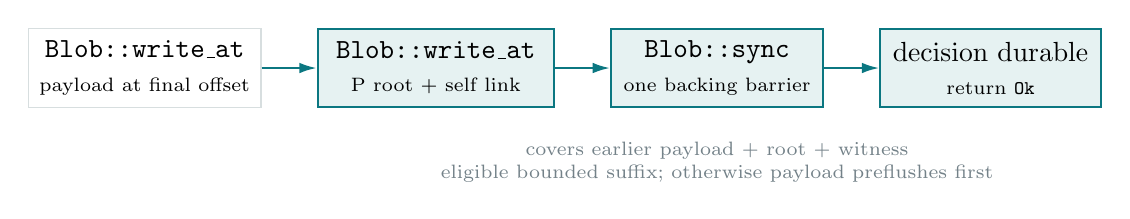
\begin{tikzpicture}[node distance=.7cm]
    \node[box,minimum width=2.7cm,minimum height=1.0cm] (append) {\texttt{Blob::write\_at}\\\scriptsize payload at final offset};
    \node[root,minimum width=3.0cm,minimum height=1.0cm,right=of append] (stage) {\texttt{Blob::write\_at}\\\scriptsize P root + self link};
    \node[root,minimum width=2.6cm,minimum height=1.0cm,right=of stage] (sync) {\texttt{Blob::sync}\\\scriptsize one backing barrier};
    \node[root,minimum width=2.5cm,minimum height=1.0cm,right=of sync] (done) {decision durable\\\scriptsize return \texttt{Ok}};
    \draw[flow] (append) -- (stage);
    \draw[flow] (stage) -- (sync);
    \draw[flow] (sync) -- (done);
    \node[below=.31cm of sync,font=\scriptsize,text=Muted,align=center] {covers earlier payload + root + witness\\eligible bounded suffix; otherwise payload preflushes first};
  \end{tikzpicture}

  \vspace{0.42cm}
  \begin{columns}[T,onlytextwidth]
    \begin{column}{0.47\textwidth}
      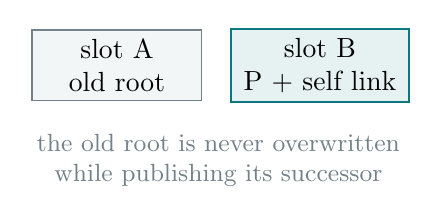
\begin{tikzpicture}
        \node[oldroot,minimum width=2.15cm] (a) {slot A\\old root};
        \node[root,minimum width=2.15cm,right=.35cm of a] (b) {slot B\\P + self link};
        \node[below=.28cm of $(a.south)!0.5!(b.south)$,font=\small,text=Muted,align=center] {the old root is never overwritten\\while publishing its successor};
      \end{tikzpicture}
    \end{column}
    \begin{column}{0.51\textwidth}
      \eyebrow{On restart}
      \begin{itemize}
        \item If the prepared root, self link, and publication-suffix CRC all validate: expose new.
        \item Otherwise: expose the preceding committed root.
        \item No follow-up P$\rightarrow$C marker and no second durability barrier.
      \end{itemize}
    \end{column}
  \end{columns}

  \vfill
  \takeaway{The self-link is the durable decision; later compatible epochs alternate and supersede it.}

  \note{The one-barrier claim is for the compatible append-only filesystem hot path. Blob::start_sync drives the same publication asynchronously. An overlapping prior decision may have to finish before a shared participant can advance. Large or non-contiguous pending epochs may also preflush immutable payload before the root is staged, but they do not copy or rewrite that payload. The generic memory publisher deliberately uses a simpler correctness-first sequence; the filesystem publisher is the one-barrier protocol path measured later.}
\end{frame}

\begin{frame}[t]{Several blobs: each root stores one link in a closed ring}
  \vspace{0.06cm}
  \begin{center}
    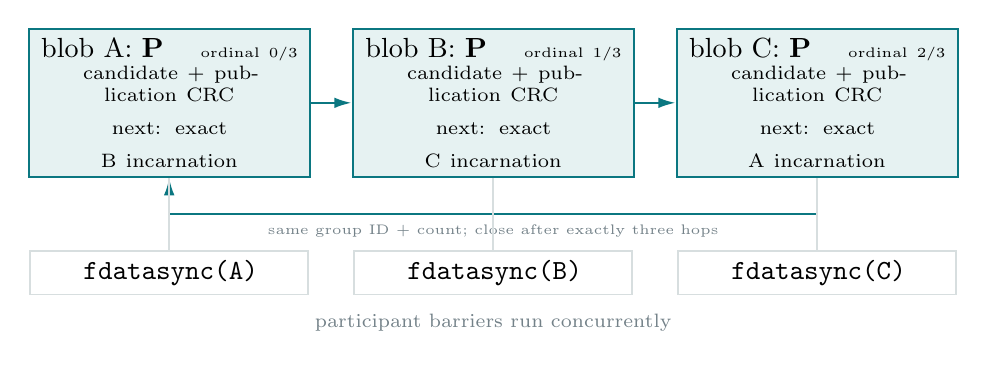
\begin{tikzpicture}[node distance=.52cm]
      \node[root,text width=3.25cm,minimum height=1.14cm] (a) {blob A: \textbf{P} \quad {\tiny ordinal 0/3}\\\scriptsize candidate + publication CRC\\next: exact B incarnation};
      \node[root,text width=3.25cm,minimum height=1.14cm,right=of a] (b) {blob B: \textbf{P} \quad {\tiny ordinal 1/3}\\\scriptsize candidate + publication CRC\\next: exact C incarnation};
      \node[root,text width=3.25cm,minimum height=1.14cm,right=of b] (c) {blob C: \textbf{P} \quad {\tiny ordinal 2/3}\\\scriptsize candidate + publication CRC\\next: exact A incarnation};
      \draw[flow] (a) -- (b);
      \draw[flow] (b) -- (c);
      \draw[flow] (c.south) -- ++(0,-.46cm) -| node[pos=.25,below,font=\tiny,text=Muted]{same group ID + count; close after exactly three hops} (a.south);

      \node[box,text width=3.25cm,minimum height=.55cm,below=.92cm of a] (sa) {\texttt{fdatasync(A)}};
      \node[box,text width=3.25cm,minimum height=.55cm,below=.92cm of b] (sb) {\texttt{fdatasync(B)}};
      \node[box,text width=3.25cm,minimum height=.55cm,below=.92cm of c] (sc) {\texttt{fdatasync(C)}};
      \draw[faintline] (a) -- (sa);
      \draw[faintline] (b) -- (sb);
      \draw[faintline] (c) -- (sc);
      \node[below=.12cm of sb,font=\scriptsize,text=Muted] {participant barriers run concurrently};
    \end{tikzpicture}
  \end{center}

  \vspace{0.2cm}
  \begin{columns}[T,onlytextwidth]
    \begin{column}{0.48\textwidth}
      \eyebrow{What one local witness carries}\par\smallskip
      \scriptsize Fresh 128-bit group ID, count + ordinal, local incarnation/candidate/removal bit, bounded publication-suffix CRC32C, and only the successor's partition/name/incarnation.
    \end{column}
    \begin{column}{0.48\textwidth}
      \eyebrow{What restart proves}\par\smallskip
      \scriptsize Opening one unresolved P follows exactly the declared ring, growing state only after each valid link. Only one unique, consecutive, closed ring can publish the complete new group.
    \end{column}
  \end{columns}

  \vspace{0.12cm}
  \centering\scriptsize Live process: one typed \texttt{Decision} in RAM. On disk: distinct local links only.

  \vfill
  \takeaway{No coordinator file and no replicated group descriptor: the participant files are the recovery index.}

  \note{The barriers are issued concurrently. The full typed decision exists only in memory while the operation is live. On disk, each root stores one local witness and one successor link. If start_apply returns Ok, all required participant states are durably recoverable, even if the completion handle is dropped. Awaiting the handle waits for activation and namespace cleanup. A failed or cancelled start remains indeterminate because every barrier may in fact have reached disk.}
\end{frame}

\begin{frame}[t]{Overlapping atomic groups}
  \vspace{0cm}
  \eyebrow{Every ring sorts participant keys: \texttt{(partition, raw blob name)}}

  \vspace{0.05cm}
  \begin{center}
    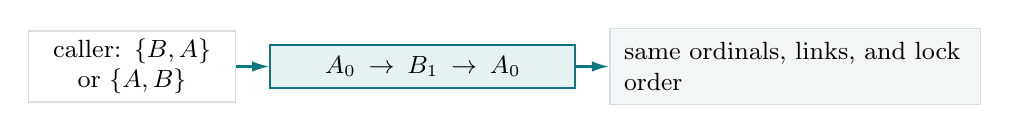
\begin{tikzpicture}[node distance=.42cm]
      \node[box,text width=2.35cm,minimum height=.54cm,font=\small] (caller) {caller: $\{B,A\}$ or $\{A,B\}$};
      \node[root,text width=3.55cm,minimum height=.54cm,right=of caller,font=\small] (ring) {$A_0 \rightarrow B_1 \rightarrow A_0$};
      \node[panel,text width=4.35cm,minimum height=.54cm,right=of ring,font=\small] (why) {same ordinals, links, and lock order};
      \draw[flow] (caller) -- (ring);
      \draw[flow] (ring) -- (why);
    \end{tikzpicture}
  \end{center}

  \vspace{0.07cm}
  \begin{columns}[T,onlytextwidth]
    \begin{column}{0.48\textwidth}
      \eyebrow{Exact participant set repeats}

      \vspace{0.05cm}
      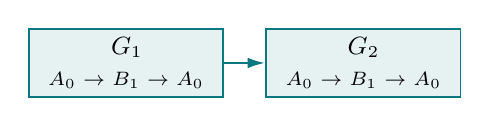
\begin{tikzpicture}[node distance=.52cm]
        \node[root,text width=2.15cm,minimum height=.78cm,font=\small] (g1) {$G_1$\\\scriptsize $A_0 \to B_1 \to A_0$};
        \node[root,text width=2.15cm,minimum height=.78cm,right=of g1,font=\small] (g2) {$G_2$\\\scriptsize $A_0 \to B_1 \to A_0$};
        \draw[flow] (g1) -- (g2);
      \end{tikzpicture}

      \vspace{0.04cm}
      \scriptsize Adjacent generations supersede directly; no P$\rightarrow$M rewrite.
    \end{column}
    \begin{column}{0.48\textwidth}
      \eyebrow{Participant set changes}

      \vspace{0.05cm}
      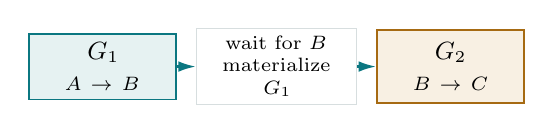
\begin{tikzpicture}[node distance=.24cm]
        \node[root,text width=1.55cm,minimum height=.78cm,font=\small] (h1) {$G_1$\\\scriptsize $A \to B$};
        \node[box,text width=1.75cm,minimum height=.78cm,right=of h1,font=\scriptsize] (wait) {wait for $B$\\materialize $G_1$};
        \node[warn,text width=1.55cm,minimum height=.78cm,right=of wait,font=\small] (h2) {$G_2$\\\scriptsize $B \to C$};
        \draw[flow] (h1) -- (wait);
        \draw[flow] (wait) -- (h2);
      \end{tikzpicture}

      \vspace{0.04cm}
      \scriptsize Shared-$B$ serialization is required; eager materialization is current policy.
    \end{column}
  \end{columns}

  \vspace{0.11cm}
  \begin{columns}[T,onlytextwidth]
    \begin{column}{0.48\textwidth}
      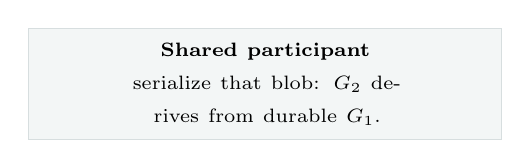
\begin{tikzpicture}
        \node[panel,text width=5.65cm,minimum height=.76cm,align=center] {\scriptsize \textbf{Shared participant}\\serialize that blob: $G_2$ derives from durable $G_1$.};
      \end{tikzpicture}
    \end{column}
    \begin{column}{0.48\textwidth}
      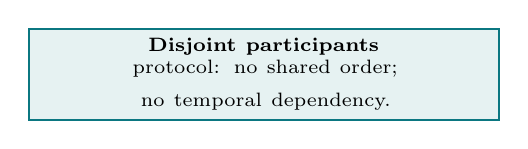
\begin{tikzpicture}
        \node[root,text width=5.65cm,minimum height=.76cm,align=center] {\scriptsize \textbf{Disjoint participants}\\protocol: no shared order;\\no temporal dependency.};
      \end{tikzpicture}
    \end{column}
  \end{columns}

  \vfill
  \takeaway{Lexicographic links and shared-blob serialization prevent cycles without imposing a storage-wide order.}

  \note{The canonical key is the partition string followed by the raw blob-name bytes. Batch canonicalization, participant lock acquisition, ordinal assignment, successor links, and recovery validation all use this order. Therefore callers may provide A,B or B,A and still produce the same ring, and overlapping batches cannot acquire the same blob locks in opposite orders. A shared blob still serializes generations: G2 cannot derive B's next root until G1 is durably committed and active. Disjoint groups have no protocol edge between them and can cross their durability frontiers in either order.}
\end{frame}

\begin{frame}[t]{Dependent writes can be built, then published together}
  \vspace{0cm}
  \eyebrow{Variable journal append: sequential staging is allowed}

  \vspace{0.08cm}
  \noindent\hfill
    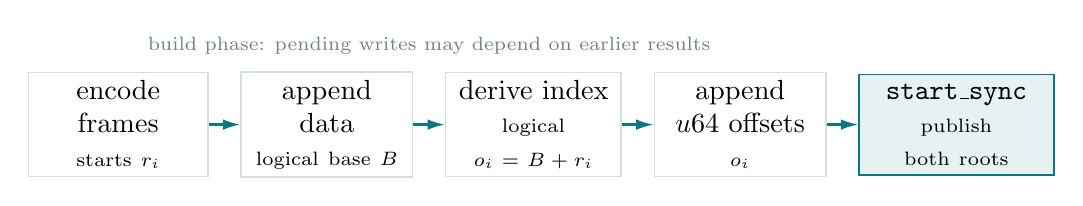
\begin{tikzpicture}[node distance=.40cm]
      \node[box,text width=2.0cm,minimum height=.72cm] (prepare) {encode frames\\\scriptsize starts $r_i$};
      \node[box,text width=1.9cm,minimum height=.72cm,right=of prepare] (data) {append data\\\scriptsize logical base $B$};
      \node[box,text width=1.95cm,minimum height=.72cm,right=of data] (derive) {derive index\\\scriptsize logical $o_i = B + r_i$};
      \node[box,text width=1.9cm,minimum height=.72cm,right=of derive] (offsets) {append $u64$ offsets\\\scriptsize $o_i$};
      \node[root,text width=2.15cm,minimum height=.72cm,right=of offsets] (publish) {\texttt{start\_sync}\\\scriptsize publish both roots};
      \draw[flow] (prepare) -- (data);
      \draw[flow] (data) -- (derive);
      \draw[flow] (derive) -- (offsets);
      \draw[flow] (offsets) -- (publish);
      \node[above=.10cm of $(prepare.north)!0.5!(offsets.north)$,font=\scriptsize,text=Muted] {build phase: pending writes may depend on earlier results};
    \end{tikzpicture}
  \hfill\null

  \vspace{0.13cm}
  \begin{columns}[T,onlytextwidth]
    \begin{column}{0.53\textwidth}
      \eyebrow{How value $i$ is located}

      \vspace{0.08cm}
      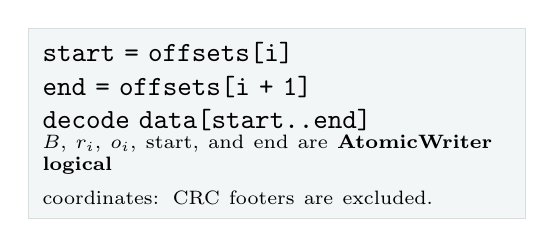
\begin{tikzpicture}
        \node[panel,text width=5.95cm,align=left] {\texttt{start = offsets[i]}\\\texttt{end = offsets[i + 1]}\\\texttt{decode data[start..end]}\\[-0.02cm]\scriptsize $B$, $r_i$, $o_i$, start, and end are \textbf{AtomicWriter logical}\\coordinates: CRC footers are excluded.};
      \end{tikzpicture}
    \end{column}
    \begin{column}{0.45\textwidth}
      \eyebrow{What becomes visible}

      \vspace{0.08cm}
      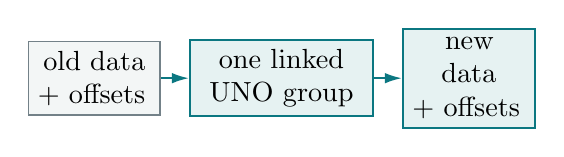
\begin{tikzpicture}[node distance=.36cm]
        \node[oldroot,text width=1.35cm,minimum height=.86cm] (oldpair) {old data\\+ offsets};
        \node[root,text width=2.0cm,minimum height=.86cm,right=of oldpair] (decision) {one linked\\UNO group};
        \node[root,text width=1.35cm,minimum height=.86cm,right=of decision] (newpair) {new data\\+ offsets};
        \draw[flow] (oldpair) -- (decision);
        \draw[flow] (decision) -- (newpair);
      \end{tikzpicture}

      \vspace{0.03cm}
      \scriptsize Restart sees the old pair or complete new pair---never mismatched data and offsets lengths.
    \end{column}
  \end{columns}

  \vfill
  \takeaway{Stage data, derive footer-free logical offsets, then publish both checked-page roots in one group.}

  \note{The batch operation is a publication boundary, not a simultaneous-write scheduler. prepare_append encodes all frames and records each relative start before I/O. AtomicWriter appends the data slice and returns its stable footer-free logical base B; the journal adds B to each relative start and appends those u64 logical offsets to the offsets writer. AtomicWriter maps those logical positions to the AtomicBlob encoded stream, whose append offsets and selected-root length include completed integrity footers. The pending writes are immediately available to the current writer but remain outside the committed roots. start_sync then creates Publish operations for both blobs in every dirty pair and starts one UNO group. If staging fails, publication never begins and the consuming MutableV2 API prevents reuse of partially mutated state. On rollover the same pattern covers the prior and current data/offsets pairs, at most four roots.}
\end{frame}

\begin{frame}[t]{Batch scale: fixed local metadata per participant}
  \vspace{0cm}
  \eyebrow{Every dirty participant: one 2 KiB slot contains its root and local witness}

  \vspace{0.07cm}
  \noindent\hfill
    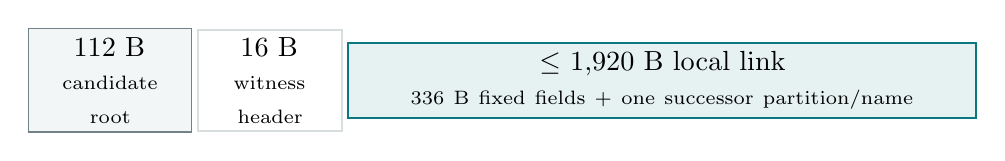
\begin{tikzpicture}[node distance=.06cm]
      \node[oldroot,text width=1.75cm,minimum height=.72cm] (roothead) {112 B\\\scriptsize candidate root};
      \node[box,text width=1.55cm,minimum height=.72cm,right=of roothead] (witness) {16 B\\\scriptsize witness header};
      \node[root,text width=7.65cm,minimum height=.72cm,right=of witness] (link) {$\leq$ 1,920 B local link\\\scriptsize 336 B fixed fields + one successor partition/name};
    \end{tikzpicture}
  \hfill\null

  \vspace{0.02cm}
  \begin{columns}[T,onlytextwidth]
    \begin{column}{0.49\textwidth}
      \eyebrow{Participant metadata}

      \vspace{0.08cm}
      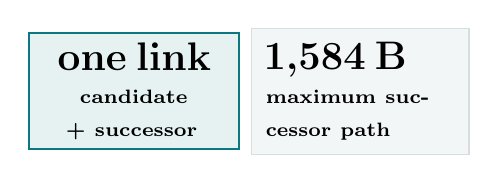
\begin{tikzpicture}[node distance=.14cm]
        \node[root,text width=2.35cm,minimum height=.78cm,align=center] (configured) {\Large\bfseries one link\\\scriptsize candidate + successor};
        \node[panel,text width=2.40cm,minimum height=.78cm,right=of configured] (encoded) {\Large\bfseries 1,584 B\\\scriptsize maximum successor path};
      \end{tikzpicture}

      \vspace{0.08cm}
      \scriptsize Each participant names only its next exact incarnation. The paths are distributed once around the ring rather than gathered into one record.
    \end{column}
    \begin{column}{0.49\textwidth}
      \eyebrow{Payload size: no protocol batch cap}

      \vspace{0.08cm}
      
\begin{tikzpicture}
        \node[root,text width=5.4cm,minimum height=.78cm] {\Large\bfseries arbitrarily large epoch\\\scriptsize streamed once + incrementally preflushed};
      \end{tikzpicture}

      \vspace{0.08cm}
      \scriptsize At most \textbf{64 MiB aggregate} remains for publication recovery CRC work. Older immutable bytes preflush while appends continue.
    \end{column}
  \end{columns}

  \vfill
  \takeaway{Metadata grows one local link per participant; payload is streamed once rather than copied.}

  \note{Every participant stores only its own candidate and one successor path. Every local link must fit its 1,920-byte witness body, leaving 1,584 bytes for the successor partition and blob name after 336 fixed bytes. The entire group name set is never encoded in one slot, so moderate names do not reduce group membership. Recovery grows state only after validating each exact successor, and installation can process a large ring in bounded chunks. An epoch may contain arbitrarily much payload within ordinary storage and offset limits. As appends arrive, completed durability operations turn older immutable bytes into a trusted prefix. Publication leaves at most 64 MiB across the group under CRC32C, so restart work stays bounded without rejecting or copying a large epoch. Fixed contiguous rollover publishes at most prior and current roots; variable publishes the data/offsets pair for each, at most four roots.}
\end{frame}

\begin{frame}[t]{Large epochs bound publication recovery work}
  \vspace{0cm}
  \eyebrow{While appending: payload is at final offsets; no candidate root exists yet}

  \vspace{0.03cm}
  \noindent\hfill
    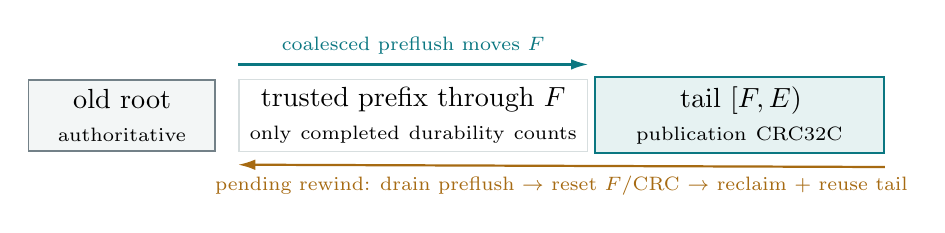
\begin{tikzpicture}[node distance=.07cm]
      \node[oldroot,text width=2.05cm,minimum height=.7cm] (old) {old root\\\scriptsize authoritative};
      \node[box,text width=4.15cm,minimum height=.7cm,right=.28cm of old] (prefix) {trusted prefix through $F$\\\scriptsize only completed durability counts};
      \node[root,text width=3.35cm,minimum height=.7cm,right=of prefix] (tail) {tail $[F,E)$\\\scriptsize publication CRC32C};
      \draw[flow] ([yshift=.18cm]prefix.north west) -- node[above,font=\scriptsize,text=Accent] {coalesced preflush moves $F$} ([yshift=.18cm]prefix.north east);
      \draw[flow,draw=Amber] ([yshift=-.16cm]tail.south east) -- node[below,font=\scriptsize,text=Amber] {pending rewind: drain preflush $\rightarrow$ reset $F$/CRC $\rightarrow$ reclaim + reuse tail} ([yshift=-.16cm]prefix.south west);
    \end{tikzpicture}
  \hfill\null

  \vspace{0cm}
  \eyebrow{At \texttt{sync}: freeze one epoch, then publish}

  \vspace{0.02cm}
  \noindent\hfill
    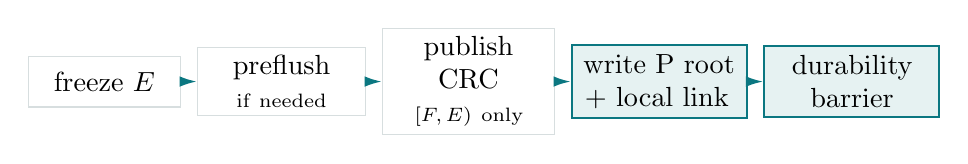
\begin{tikzpicture}[node distance=.2cm]
      \node[box,text width=1.65cm,minimum height=.64cm] (freeze) {freeze $E$};
      \node[box,text width=1.85cm,minimum height=.64cm,right=of freeze] (wait) {preflush\\\scriptsize if needed};
      \node[box,text width=1.9cm,minimum height=.64cm,right=of wait] (crc) {publish CRC\\\scriptsize $[F,E)$ only};
      \node[root,text width=1.9cm,minimum height=.64cm,right=of crc] (stage) {write P root\\+ local link};
      \node[root,text width=1.9cm,minimum height=.64cm,right=of stage] (barrier) {durability\\barrier};
      \draw[flow] (freeze) -- (wait);
      \draw[flow] (wait) -- (crc);
      \draw[flow] (crc) -- (stage);
      \draw[flow] (stage) -- (barrier);
    \end{tikzpicture}
  \hfill\null

  \vspace{0cm}
  \eyebrow{Crash outcome}

  \vspace{0cm}
  \noindent\hfill
    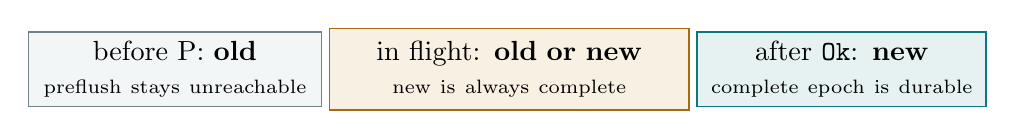
\begin{tikzpicture}[node distance=.08cm]
      \node[oldroot,text width=3.4cm,minimum height=.58cm] (before) {before P: \textbf{old}\\\scriptsize preflush stays unreachable};
      \node[warn,text width=4.25cm,minimum height=.58cm,right=of before] (during) {in flight: \textbf{old or new}\\\scriptsize new is always complete};
      \node[root,text width=3.35cm,minimum height=.58cm,right=of during] (after) {after \texttt{Ok}: \textbf{new}\\\scriptsize complete epoch is durable};
    \end{tikzpicture}
  \hfill\null

  \vfill
  \takeaway{Repeat per participant: no payload-byte cap, at most 64 MiB aggregate restart tail, and concurrent final barriers.}

  \note{Only a completed fdatasync-equivalent advances the trusted frontier F; sync_file_range or another writeback hint never does. Background preflush is coalesced while the producer continues, and it writes no root. At publication, each participant waits only for any durability frontier it must rely on. Its local witness names that trusted prefix and carries CRC32C for the remaining tail; tail budgets sum to at most 64 MiB across the group. This publication checksum is independent of the long-lived integrity-unit footer or open-unit CRC. The final participant barriers run concurrently. A very large append followed immediately by sync may still wait for a payload preflush and then the root barrier, but payload is never copied or written twice. Before root staging, a crash can expose only old. Once staging begins, the ordinary indeterminate window applies: old or complete new.}
\end{frame}

\begin{frame}[t]{Independent groups have no temporal dependency}
  \vspace{0.03cm}
  \begin{columns}[T,onlytextwidth]
    \begin{column}{0.56\textwidth}
      \eyebrow{Independent groups}

      \vspace{0.14cm}
      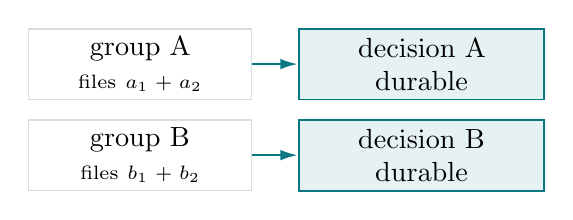
\begin{tikzpicture}[node distance=.58cm]
        \node[box,text width=2.55cm,minimum height=.62cm] (a) {group A\\\scriptsize files $a_1 + a_2$};
        \node[root,text width=2.8cm,right=of a] (ad) {decision A durable};
        \draw[flow] (a) -- (ad);

        \node[box,text width=2.55cm,minimum height=.62cm,below=.24cm of a] (b) {group B\\\scriptsize files $b_1 + b_2$};
        \node[root,text width=2.8cm,right=of b] (bd) {decision B durable};
        \draw[flow] (b) -- (bd);
      \end{tikzpicture}
    \end{column}
    \begin{column}{0.42\textwidth}
      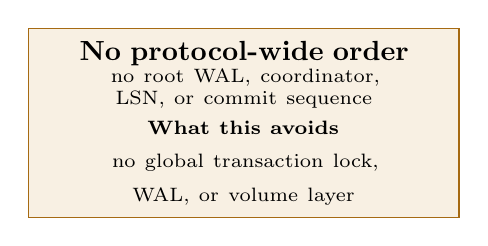
\begin{tikzpicture}
        \node[warn,text width=5.15cm] {\textbf{No protocol-wide order}\\\scriptsize no root WAL, coordinator, LSN, or commit sequence\\[.1cm]\textbf{What this avoids}\\\scriptsize no global transaction lock, WAL, or volume layer};
      \end{tikzpicture}
    \end{column}
  \end{columns}

  \vspace{0.12cm}
  \eyebrow{Crash states for independently started A and B}

  \vspace{0.06cm}
  \noindent\hfill\small old A / old B
  \quad $\vert$ \quad new A / old B
  \quad $\vert$ \quad \textcolor{Amber}{\textbf{old A / new B is possible}}
  \quad $\vert$ \quad new A / new B\hfill\null

  \vspace{0.14cm}
  \eyebrow{When B has a temporal dependency on A}

  \vspace{0.03cm}
  \noindent\hfill
    
\begin{tikzpicture}[node distance=.72cm]
      \node[box,text width=2.25cm] (pa) {publish A};
      \node[root,text width=3.0cm,right=of pa] (da) {A's decision is durable};
      \node[box,text width=2.25cm,right=of da] (pb) {then publish B};
      \draw[flow] (pa) -- (da);
      \draw[flow] (da) -- (pb);
      \node[right=.75cm of pb,font=\scriptsize,text=Accent,align=left] {old/old, new/old, new/new\\\textbf{never old A / new B}};
    \end{tikzpicture}
  \hfill\null

  \vfill
  \takeaway{Independent groups are independent; encode a real dependency in one group or wait for the earlier durable edge.}

  \note{Two disjoint start_apply calls have no shared sequence number; the protocol permits their durable frontiers to cross in either order. Current backends may serialize namespace work as an implementation constraint, but that creates no semantic dependency. UNO does not interpose a global transaction lock, WAL, or volume-like layer on ordinary blobs. Opening one participant follows and repairs only its exact linked ring; recovery does not scan or order unrelated groups. If B semantically depends on A, either stage both pending mutations and publish them in one group, or do not begin B's separate group until A's durable decision is proven. start_apply returning Ok proves durability; awaiting its handle additionally waits for activation and namespace cleanup. A workload that truly needs one total order can still add a higher-level root WAL.}
\end{frame}

\begin{frame}[t]{Boundary: Freezer materializations stay ordinary}
  \vspace{0cm}
  \eyebrow{Immutable Archive is composite: only authority needs append-only atomic publication}

  \vspace{0cm}
  \begin{columns}[T,onlytextwidth]
    \begin{column}{0.48\textwidth}
      \eyebrow{Not converted in place}

      \vspace{0.03cm}
      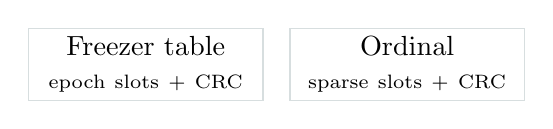
\begin{tikzpicture}[node distance=.32cm]
        \node[box,text width=2.7cm,minimum height=.64cm] (table) {Freezer table\\\scriptsize epoch slots + CRC};
        \node[box,text width=2.7cm,minimum height=.64cm,right=of table] (ordinal) {Ordinal\\\scriptsize sparse slots + CRC};
      \end{tikzpicture}

      \vspace{0.02cm}
      \scriptsize These tables overwrite slots. Their local CRCs detect damage but cannot roll bytes back.
    \end{column}
    \begin{column}{0.50\textwidth}
      \eyebrow{Append-only pieces can participate}

      \vspace{0.03cm}
      
\begin{tikzpicture}[node distance=.46cm]
        \node[root,text width=2.65cm,minimum height=.64cm] (values) {value journal\\\scriptsize append-only payload};
        \node[root,text width=2.7cm,minimum height=.64cm,right=of values] (index) {key-index journal\\\scriptsize returned locations};
        \draw[flow] (values) -- (index);
      \end{tikzpicture}

      \vspace{0.02cm}
      \scriptsize Journals and an archive-state authority can move together.
    \end{column}
  \end{columns}

  \vspace{0cm}
  \eyebrow{Logical commit with one explicit temporal dependency}

  \vspace{0.03cm}
  \noindent\hfill
    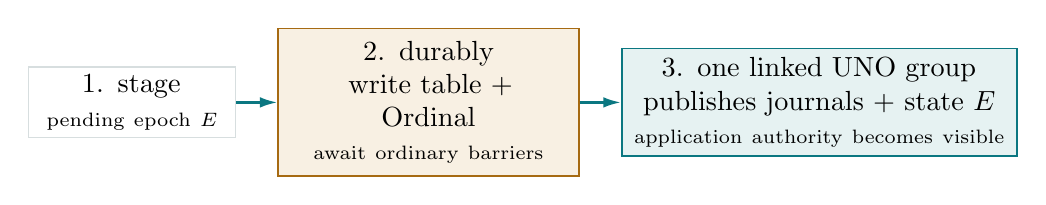
\begin{tikzpicture}[node distance=.52cm]
      \node[box,text width=2.35cm,minimum height=.66cm] (stage) {1. stage\\\scriptsize pending epoch $E$};
      \node[warn,text width=3.5cm,minimum height=.66cm,right=of stage] (materialize) {2. durably write table +\\Ordinal\\\scriptsize await ordinary barriers};
      \node[root,text width=4.7cm,minimum height=.66cm,right=of materialize] (publish) {3. one linked UNO group publishes journals + state $E$\\\scriptsize application authority becomes visible};
      \draw[flow] (stage) -- (materialize);
      \draw[flow] (materialize) -- (publish);
    \end{tikzpicture}
  \hfill\null

  \vspace{0cm}
  \noindent\hfill
    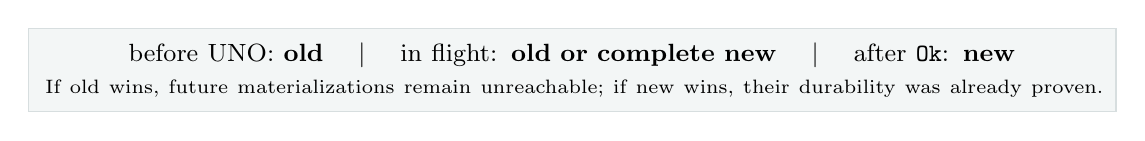
\begin{tikzpicture}
      \node[panel,text width=13.45cm,align=center] {\small before UNO: \textbf{old} \quad $\vert$ \quad in flight: \textbf{old or complete new} \quad $\vert$ \quad after \texttt{Ok}: \textbf{new}\\[-.01cm]\scriptsize If old wins, future materializations remain unreachable; if new wins, their durability was already proven.};
    \end{tikzpicture}
  \hfill\null

  \vfill
  \takeaway{Ordinary materializations may be written and made durable before UNO publishes the authority that reaches them.}

  \note{The Freezer table's alternating epoch/checksum slots and Ordinal's sparse in-place records are not AtomicBlob candidates. A composite Archive design can stage append-only value and key-index journals, write the future table and Ordinal materializations, and await their ordinary durability handles. Only then may it publish journal roots plus an AtomicBlob archive-state snapshot carrying the Freezer checkpoint and ordinal bitmaps. A crash before UNO leaves the old authority in force; future materializations remain unreachable. If the new authority wins, their durability was already proven. This boundary does not turn UNO into a global coordinator or general overwrite engine.}
\end{frame}

\begin{frame}[t]{Recovery is correct for arbitrary surviving write subsets}
  \vspace{0cm}
  {\centering\scriptsize P = prepared linked candidate \quad M = materialized retained root \quad T = durable tombstone\par}

  \vspace{0.08cm}
  \scriptsize
  \renewcommand{\arraystretch}{1.2}
  \begin{tabularx}{\textwidth}{>{\raggedright\arraybackslash}p{3.6cm} >{\raggedright\arraybackslash}p{4.55cm} X}
    \toprule
    \textbf{What validates after restart} & \textbf{What recovery can prove} & \textbf{Exposed result} \\
    \midrule
    No M/T proof; every exact P, local link, incarnation, candidate, and publication suffix validates & One group ID/count; unique consecutive ordinals close after exactly $N$ hops & New roots for the whole group \\
    No M/T proof; any P, link, incarnation, candidate, or publication suffix is missing/mismatched & The linked group decision is incomplete & Old roots for the whole group \\
    An exact materialized M or tombstone T validates & Installation began only after the P ring was durable & Finish peers; after unlink begins, resume the descending frontier from ordinal 0 \\
    \bottomrule
  \end{tabularx}

  \vspace{0.22cm}
  \begin{columns}[T,onlytextwidth]
    \begin{column}{0.32\textwidth}
      \eyebrow{Torn roots}\par\smallskip
      \scriptsize Root and witness-envelope checksums reject mixed spellings and partial installation. P is not a final standalone root.
    \end{column}
    \begin{column}{0.32\textwidth}
      \eyebrow{Torn payload}\par\smallskip
      \scriptsize A trusted prefix plus publication CRC32C rejects partial visibility with probabilistic checksum assurance.
    \end{column}
    \begin{column}{0.32\textwidth}
      \eyebrow{Threat boundary}\par\smallskip
      \scriptsize CRC32C detects crash damage on trusted local disk; it is not tamper authentication.
    \end{column}
  \end{columns}

  \vfill
  \takeaway{The protocol never assumes that surviving writes form a prefix in submission order.}

  \note{This is the central correctness argument. Unsynchronized writes can survive in any combination, not merely a submission-order prefix. The old roots remain self-contained. A new group is selected only from one complete closed ring of exact, checksummed local evidence, or from a later materialized/tombstone proof that makes roll-forward mandatory. The publication-suffix checksum is only for deciding whether a speculative candidate survived; long-lived payload reads use integrity-unit checks instead.}
\end{frame}

\begin{frame}[t]{Append is the fast path; delete is ordered by phase}
  \vspace{0.03cm}
  \begin{columns}[T,onlytextwidth]
    \begin{column}{0.32\textwidth}
      \eyebrow{Append}
      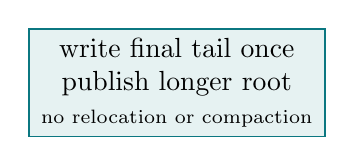
\begin{tikzpicture}
        \node[root,minimum width=3.65cm,minimum height=1.18cm] {write final tail once\\publish longer root\\\scriptsize no relocation or compaction};
      \end{tikzpicture}
    \end{column}
    \begin{column}{0.32\textwidth}
      \eyebrow{Rewind}
      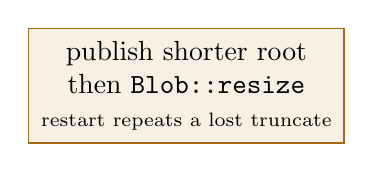
\begin{tikzpicture}
        \node[warn,minimum width=3.65cm,minimum height=1.18cm] {publish shorter root\\then \texttt{Blob::resize}\\\scriptsize restart repeats a lost truncate};
      \end{tikzpicture}
    \end{column}
    \begin{column}{0.32\textwidth}
      \eyebrow{Delete}
      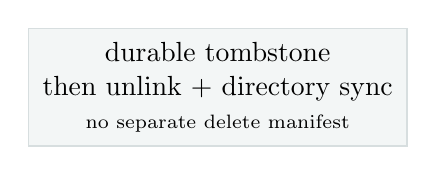
\begin{tikzpicture}
        \node[panel,minimum width=3.65cm,minimum height=1.18cm,align=center] {durable tombstone\\then unlink + directory sync\\\scriptsize no separate delete manifest};
      \end{tikzpicture}
    \end{column}
  \end{columns}

  \vspace{0.05cm}
  \eyebrow{Group delete: finish the ring walk before changing the namespace}

  \vspace{0.12cm}
  \begin{center}
    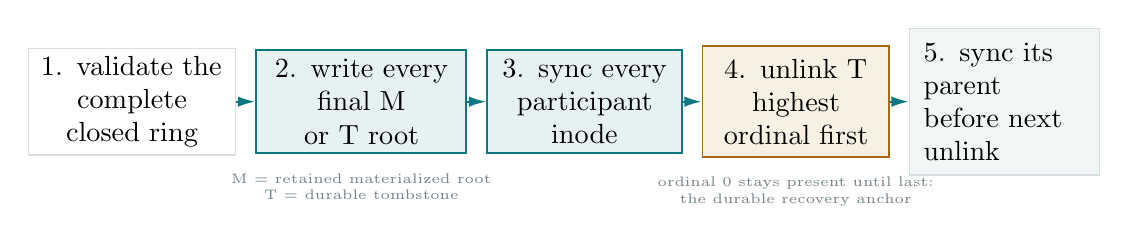
\begin{tikzpicture}[node distance=.24cm]
      \node[box,text width=2.35cm,minimum height=.76cm] (walk) {1. validate the\\complete closed ring};
      \node[root,text width=2.35cm,minimum height=.76cm,right=of walk] (materialize) {2. write every\\final M or T root};
      \node[root,text width=2.15cm,minimum height=.76cm,right=of materialize] (sync) {3. sync every\\participant inode};
      \node[warn,text width=2.05cm,minimum height=.76cm,right=of sync] (unlink) {4. unlink T\\highest ordinal first};
      \node[panel,text width=2.05cm,minimum height=.76cm,right=of unlink] (dir) {5. sync its parent\\before next unlink};
      \draw[flow] (walk) -- (materialize);
      \draw[flow] (materialize) -- (sync);
      \draw[flow] (sync) -- (unlink);
      \draw[flow] (unlink) -- (dir);
      \node[below=.12cm of materialize,font=\tiny,text=Muted,align=center] {M = retained materialized root\\T = durable tombstone};
      \node[below=.12cm of unlink,font=\tiny,text=Muted,align=center] {ordinal 0 stays present until last:\\the durable recovery anchor};
    \end{tikzpicture}
  \end{center}

  \vspace{0.12cm}
  \small Rewind keeps the old root as rollback until the shorter root is durable. After delete step 3, each M is independent; descending durable unlinks keep every remaining T reachable from ordinal 0.

  \vfill
  \takeaway{All final roots first; then a durable descending unlink frontier. Ordinal 0 replaces a delete manifest.}

  \note{A rewind that crosses the committed frontier fences new appends until synchronization publishes the shorter root. Physical truncation happens afterward through Blob::resize; if that truncate is lost, the shorter durable root makes reopen repeat it before discarded offsets can be reused. Delete has namespace durability work and is not the same cheap write-only path. Recovery first follows and validates the whole linked ring. It then materializes retained roots as M and deleted roots as T, and completes every participant durability barrier before unlinking any T. Tombstones are unlinked from the highest ordinal toward zero, with the parent directory synchronized after each unlink. Therefore a crash leaves a resumable descending frontier. A recreated same-name path has a different incarnation and is never removed.}
\end{frame}

\begin{frame}[t]{Migration stays inside initialization}
  \vspace{0.02cm}
  \eyebrow{The storage primitive migrates one quiesced name at a time}

  \vspace{0.08cm}
  \begin{center}
    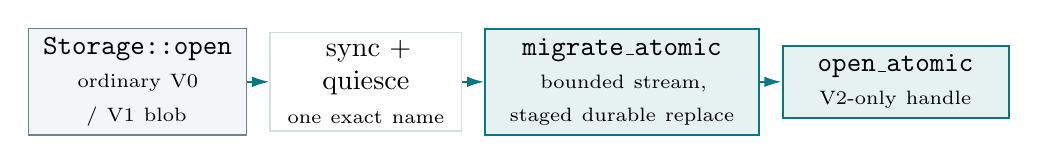
\begin{tikzpicture}[node distance=.28cm]
      \node[oldroot,text width=2.45cm,minimum height=.78cm] (ordinary) {\texttt{Storage::open}\\\scriptsize ordinary V0 / V1 blob};
      \node[box,text width=2.15cm,minimum height=.78cm,right=of ordinary] (quiesce) {sync + quiesce\\\scriptsize one exact name};
      \node[root,text width=3.15cm,minimum height=.78cm,right=of quiesce] (migrate) {\texttt{migrate\_atomic}\\\scriptsize bounded stream, staged durable replace};
      \node[root,text width=2.55cm,minimum height=.78cm,right=of migrate] (atomic) {\texttt{open\_atomic}\\\scriptsize V2-only handle};
      \draw[flow] (ordinary) -- (quiesce);
      \draw[flow] (quiesce) -- (migrate);
      \draw[flow] (migrate) -- (atomic);
    \end{tikzpicture}
  \end{center}

  \vspace{0.16cm}
  \begin{columns}[T,onlytextwidth]
    \begin{column}{0.48\textwidth}
      \eyebrow{Explicit and resumable}
      \small
      \begin{itemize}\setlength\itemsep{0.03cm}
        \item Ordinary \texttt{Storage} formats do not migrate implicitly; \texttt{open\_atomic} rejects an ordinary blob.
        \item The filesystem copy uses bounded memory, synchronizes the staged inode, durably replaces the exact generation, and is safe to retry.
      \end{itemize}
    \end{column}
    \begin{column}{0.50\textwidth}
      \eyebrow{Contiguous init}
      \small
      \begin{itemize}\setlength\itemsep{0.03cm}
        \item Legacy checked pages have different framing, so init decodes and re-encodes one section blob at a time into native checked pages.
        \item Only init sees mixed state. A successful call returns fixed or variable application code that uses V2 exclusively.
      \end{itemize}
    \end{column}
  \end{columns}

  \vfill
  \takeaway{Migration is a bounded init-time bridge, not a compatibility branch in the steady-state journal.}

  \note{The generic AtomicStorage migration preserves the application's blob version and logical bytes. On filesystems it streams through a staged native V2 inode with bounded memory and an exact durable replacement; retry resolves an interrupted replace or directory-sync window. Contiguous cannot use only that outer-layout copy because its legacy physical pages carry a different footer. Its init path therefore runs legacy recovery, replays logical items into native Chunked checked pages one section at a time, durably stages each replacement before pruning its source, and finally publishes the start marker. A small temporary witness makes that conversion resumable, but it is removed before init returns and is not part of steady-state recovery.}
\end{frame}

\begin{frame}[t]{Contiguous V2 drops the \texttt{Metadata} checkpoint}
  \vspace{0.02cm}
  \begin{columns}[T,onlytextwidth]
    \begin{column}{0.43\textwidth}
      \eyebrow{Before}

      \vspace{0.12cm}
      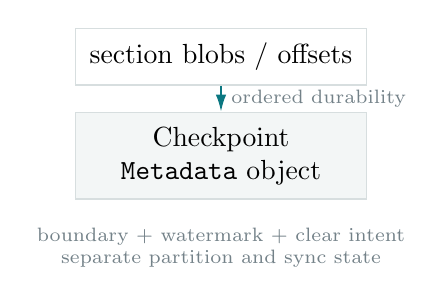
\begin{tikzpicture}[node distance=.33cm]
        \node[box,minimum width=3.7cm] (sections) {section blobs / offsets};
        \node[panel,minimum width=3.7cm,below=of sections,align=center] (checkpoint) {Checkpoint\\\texttt{Metadata} object};
        \draw[flow] (sections) -- node[right,font=\scriptsize,text=Muted]{ordered durability} (checkpoint);
        \node[below=.24cm of checkpoint,font=\scriptsize,text=Muted,align=center] {boundary + watermark + clear intent\\separate partition and sync state};
      \end{tikzpicture}
    \end{column}
    \begin{column}{0.55\textwidth}
      \eyebrow{Native V2 steady state}

      \vspace{0.12cm}
      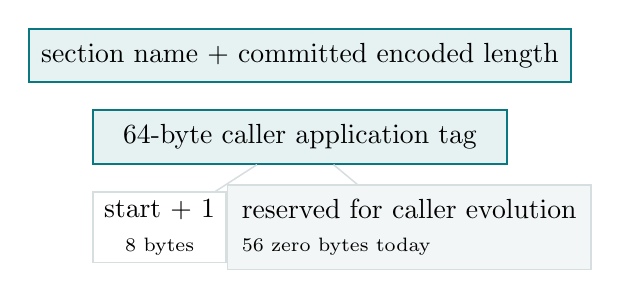
\begin{tikzpicture}[node distance=.33cm]
        \node[root,minimum width=5.25cm] (section) {section name + committed encoded length};
        \node[root,minimum width=5.25cm,below=of section] (tag) {64-byte caller application tag};
        \node[box,minimum width=1.65cm,below=.34cm of tag.south west,anchor=north west] (start) {start + 1\\\scriptsize 8 bytes};
        \node[panel,minimum width=3.6cm,right=0cm of start] (available) {reserved for caller evolution\\\scriptsize 56 zero bytes today};
        \draw[faintline] (tag) -- (start);
        \draw[faintline] (tag) -- (available);
      \end{tikzpicture}
    \end{column}
  \end{columns}

  \vspace{0.06cm}
  \scriptsize
  \begin{itemize}\setlength\itemsep{0.04cm}
    \item Both fixed and variable contiguous use \textbf{\texttt{Chunked(4092)}} checked pages: 4,092 logical bytes + a V2-owned 4-byte footer.
    \item Variable V2 stages data first, derives logical offsets, then publishes matching data + offsets roots in the \textbf{same UNO group}.
    \item One fixed section or variable pair holds start + 1; page geometry maps encoded lengths to logical bounds.
    \item \texttt{MutableV2}: consuming mutations, \texttt{start\_sync}, and \texttt{sync}---no legacy \texttt{commit} split.
  \end{itemize}

  \vfill
  \takeaway{Offsets remain as the variable index; the separate checkpoint object disappears.}

  \note{This is the direct contiguous payoff. We do not encode more journal frames just to recover the start. In native steady state the first eight tag bytes hold big-endian start + 1, all zero means no active start, and the remaining 56 bytes must be zero. Integrity state consumes none of the caller tag; it lives in dedicated root fields. Both journal kinds use AtomicWriter with Chunked(4092), despite the name ``variable journal.'' Caller-delimited IntegrityScheme::Variable is a separate generic AtomicBlob facility. Consuming mutation methods prevent reuse after failed or cancelled storage operations, while snapshots remain available for concurrent readers.}
\end{frame}

\begin{frame}[t]{Checked pages: immutable footer, bounded open tail}
  \vspace{0cm}
  \begin{columns}[T,onlytextwidth]
    \begin{column}{0.52\textwidth}
      \eyebrow{\texttt{Chunked(4092)} encoding}

      \vspace{0.05cm}
      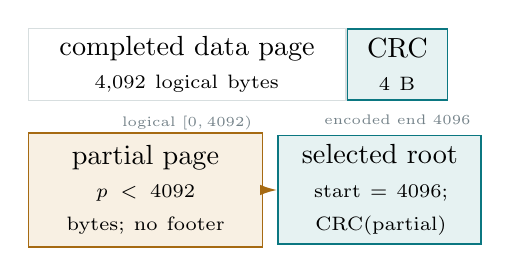
\begin{tikzpicture}[node distance=0cm]
        \node[box,text width=3.75cm,minimum height=.64cm] (page) {completed data page\\\scriptsize 4,092 logical bytes};
        \node[root,text width=.95cm,minimum height=.64cm,right=of page] (footer) {CRC\\\scriptsize 4 B};
        \node[below=.06cm of page,font=\tiny,text=Muted] {logical $[0,4092)$};
        \node[below=.06cm of footer,font=\tiny,text=Muted] {encoded end 4096};

        \node[warn,text width=2.65cm,minimum height=.6cm,below=.39cm of page.south west,anchor=north west] (tail) {partial page\\\scriptsize $p<4092$ bytes; no footer};
        \node[root,text width=2.25cm,minimum height=.6cm,right=.18cm of tail] (rootcrc) {selected root\\\scriptsize start = 4096; CRC(partial)};
        \draw[flow,draw=Amber] (tail) -- (rootcrc);
      \end{tikzpicture}

      \vspace{0.04cm}
      \scriptsize \texttt{sync} stores the partial page's start and rolling CRC in the root without closing it. At 4,092 bytes, V2 appends the footer and the 4,096-byte encoded page becomes immutable.
    \end{column}
    \begin{column}{0.46\textwidth}
      \eyebrow{Current and planned reads}

      \vspace{0.03cm}
      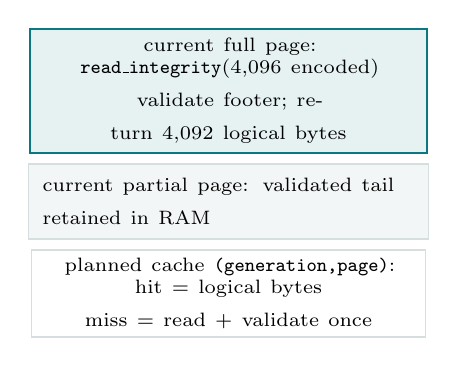
\begin{tikzpicture}[node distance=.12cm]
        \node[root,text width=4.72cm,minimum height=.5cm] (full) {\scriptsize current full page: \texttt{read\_integrity}(4,096 encoded)\\validate footer; return 4,092 logical bytes};
        \node[panel,text width=4.72cm,minimum height=.44cm,below=of full] (ramtail) {\scriptsize current partial page: validated tail retained in RAM};
        \node[box,text width=4.72cm,minimum height=.5cm,below=of ramtail] (cache) {\scriptsize planned cache \texttt{(generation,page)}: hit = logical bytes\\miss = read + validate once};
      \end{tikzpicture}

      \vspace{0.02cm}
      \scriptsize Today cache-only reads miss. The plan coalesces faults; rewind invalidates the shortened page and suffix.
    \end{column}
  \end{columns}

  \vspace{0.02cm}
  
\begin{tikzpicture}
    \node[panel,text width=13.45cm,align=center,inner ysep=.05cm] {\tiny \textbf{Coordinates:} \texttt{AtomicBlob} $e$ is encoded and includes footers; \texttt{AtomicWriter}/journal $l$ is logical and excludes them. Backing = $4096+e$; filesystem = $8192+e$.};
  \end{tikzpicture}

  \vfill
  \takeaway{The root protects the open page; every completed page has an immutable footer and is lazily cacheable.}

  \note{This is the complete checked-page model on one slide. Both contiguous implementations use AtomicWriter with a 4,092-byte logical page and a four-byte V2 footer. Small appends extend one open page across any number of syncs. The selected root carries that open page's encoded start and rolling CRC32C; its bytes have no footer yet. AtomicWriter retains and validates the partial tail when it opens. Historical complete pages are read lazily with read_integrity, which consumes and validates the footer before returning only logical bytes. Current V2 has no CacheRef integration; the lower flow is a plan. A future cache keys complete pages by exact blob generation and page, validates a miss once, stores only the 4,092 logical bytes, keeps the partial tail private, and invalidates the shortened page and suffix on rewind.}
\end{frame}

\begin{frame}[t]{CRC32C has four separate jobs}
  \vspace{0cm}
  \begin{columns}[T,onlytextwidth]
    \begin{column}{0.24\textwidth}
      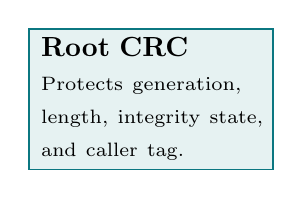
\begin{tikzpicture}
        \node[root,text width=2.78cm,minimum height=.88cm,align=left] {\textbf{Root CRC}\\\scriptsize Protects generation, length, integrity state, and caller tag.};
      \end{tikzpicture}
    \end{column}
    \begin{column}{0.24\textwidth}
      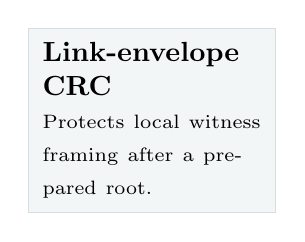
\begin{tikzpicture}
        \node[panel,text width=2.78cm,minimum height=.88cm,align=left] {\textbf{Link-envelope CRC}\\\scriptsize Protects local witness framing after a prepared root.};
      \end{tikzpicture}
    \end{column}
    \begin{column}{0.24\textwidth}
      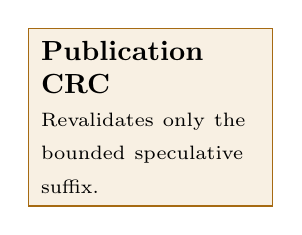
\begin{tikzpicture}
        \node[warn,text width=2.78cm,minimum height=.88cm,align=left] {\textbf{Publication CRC}\\\scriptsize Revalidates only the bounded speculative suffix.};
      \end{tikzpicture}
    \end{column}
    \begin{column}{0.24\textwidth}
      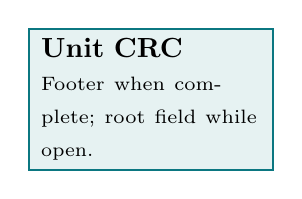
\begin{tikzpicture}
        \node[root,text width=2.78cm,minimum height=.88cm,align=left] {\textbf{Unit CRC}\\\scriptsize Footer when complete; root field while open.};
      \end{tikzpicture}
    \end{column}
  \end{columns}

  \vspace{0.08cm}
  \eyebrow{The generic integrity API chooses unit boundaries; callers still own indexes}

  \vspace{0.02cm}
  \begin{columns}[T,onlytextwidth]
    \begin{column}{0.32\textwidth}
      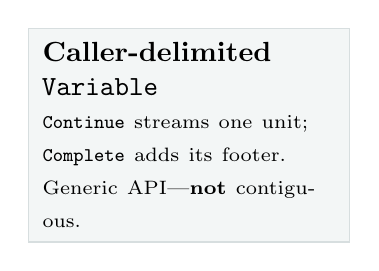
\begin{tikzpicture}
        \node[panel,text width=3.72cm,minimum height=.82cm,align=left] {\textbf{Caller-delimited \texttt{Variable}}\\\scriptsize \texttt{Continue} streams one unit; \texttt{Complete} adds its footer. Generic API---\textbf{not} contiguous.};
      \end{tikzpicture}
    \end{column}
    \begin{column}{0.32\textwidth}
      \begin{tikzpicture}
        \node[root,text width=3.72cm,minimum height=.82cm,align=left] {\textbf{\texttt{Chunked(n)}}\\\scriptsize Closes every $n$ data bytes. Both contiguous forms bind $n=4092$.};
      \end{tikzpicture}
    \end{column}
    \begin{column}{0.32\textwidth}
      \begin{tikzpicture}
        \node[panel,text width=3.72cm,minimum height=.82cm,align=left] {\textbf{Read / rewind}\\\scriptsize Validate one unit; rewind rebuilds the retained open-unit CRC when needed.};
      \end{tikzpicture}
    \end{column}
  \end{columns}

  \vspace{0.04cm}
  {\centering\tiny A compare token fences stale integrity writers before payload I/O; raw \texttt{Blob::read\_at} exposes encoded bytes without unit validation.\par}

  \vfill
  \takeaway{CRC32C rejects accidental crash damage probabilistically; it is neither authentication nor rollback material.}

  \note{Do not collapse these checksum roles. The root CRC covers root metadata. The witness-envelope CRC covers the locally embedded link framing. The publication checksum proves only that a bounded candidate suffix survived well enough to select an old or new epoch; it is not permanent read validation. Integrity-unit checks protect later payload reads: a completed unit has an immediate four-byte footer, while the selected root carries the start and checksum of the only unfinished unit. The API begins Unbound. Complete binds generic Variable; Chunked binds one fixed width; the durable scheme cannot later change. Variable deliberately stores no index of completed unit boundaries, so the caller must remember its own offsets. Tokens serialize immediately visible integrity and tag state.}
\end{frame}

\begin{frame}[t]{Reopen cost is bounded at both layers}
  \vspace{0cm}
  \begin{columns}[T,onlytextwidth]
    \begin{column}{0.6\textwidth}
      \eyebrow{Crossing many fixed sections in one epoch}

      \vspace{0.04cm}
      \begin{tikzpicture}[node distance=.24cm,scale=.75,transform shape]
        \node[root,minimum width=2.0cm] (prior) {prior authority\\\scriptsize marker set};
        \node[box,minimum width=1.85cm,right=.45cm of prior] (s1) {sealed 1\\\scriptsize unmarked};
        \node[box,minimum width=1.85cm,right=of s1] (s2) {sealed 2\\\scriptsize unmarked};
        \node[box,minimum width=1.85cm,right=of s2] (sn) {$\cdots$};
        \node[root,minimum width=2.0cm,right=of sn] (tail) {current tail\\\scriptsize marker set};
        \draw[flow] (prior) -- (s1);
        \draw[flow] (s1) -- (s2);
        \draw[flow] (s2) -- (sn);
        \draw[flow] (sn) -- (tail);
        \node[panel,below=.62cm of s2,minimum width=3.9cm,align=center] (decision) {final UNO group\\\scriptsize prior authority + current tail only};
        \draw[plainline] (prior.south) |- (decision.west);
        \draw[plainline] (tail.south) |- (decision.east);
      \end{tikzpicture}

      \vspace{0.06cm}
      \small Sealed intermediate sections may be durably staged while unreachable; their names fill the interval once the marker publishes.

      \vspace{0.04cm}
      \begin{tikzpicture}
        \node[panel,text width=6.65cm,align=center] {\small fixed: \textbf{2 roots}\qquad variable: \textbf{4 roots}\\\scriptsize prior/current $\times$ data/offsets, all in one group};
      \end{tikzpicture}
    \end{column}
    \begin{column}{0.38\textwidth}
      \eyebrow{Open / restart path}

      \vspace{0.04cm}
      \begin{tikzpicture}[node distance=.19cm]
        \node[box,minimum width=4.35cm] (names) {scan section names};
        \node[box,minimum width=4.35cm,below=of names] (roots) {namespace recovery, if needed\\\scriptsize follow one exact declared P ring};
        \node[root,minimum width=4.35cm,below=of roots] (bounds) {raw \texttt{AtomicBlob} core\\\scriptsize read exactly two root headers; no payload};
        \node[panel,minimum width=4.35cm,below=of bounds] (writers) {construct checked-page writers\\\scriptsize validate retained partial tails};
        \draw[flow] (names) -- (roots);
        \draw[flow] (roots) -- (bounds);
        \draw[flow] (bounds) -- (writers);
      \end{tikzpicture}

      \vspace{0cm}
      \scriptsize Fixed: $\leq 1$ tail per retained section. Variable: sealed pairs are complete; active data + offsets: $\leq 2$ tails. Full pages remain lazy.
    \end{column}
  \end{columns}

  \vfill
  \takeaway{Raw core reads two root slots; higher layers validate only bounded partial tails.}

  \note{The bounded final group is the important rollover optimization. Sealed intermediate sections can be staged durably while unreachable. The one movable authority marker makes all names between the retained start and active tail reachable at once. The variable journal needs four roots because both data and offsets for the prior authority and current tail must move together; this journal name is unrelated to IntegrityScheme::Variable. The raw UNO core recovery itself reads exactly the two fixed root headers and never reads an unfinished unit or completed footer. Filesystem namespace recovery is a separate bounded step that may follow one exact unresolved P ring and validate its bounded publication suffix. Contiguous init then constructs AtomicWriter instances: fixed may validate one bounded partial Chunked tail for every retained section, while sealed variable pairs are page-complete and only the active data and offsets writers may each validate a tail. Completed pages remain lazy.}
\end{frame}

\begin{frame}[t]{Benchmark method: paired ordinary blobs vs UNO}
  \vspace{0cm}
  \eyebrow{One operation = four independent 4 MiB contiguous appends}

  \vspace{0.05cm}
  \begin{columns}[T,onlytextwidth]
    \begin{column}{0.49\textwidth}
      \begin{tikzpicture}[node distance=.22cm]
        \node[oldroot,text width=5.65cm,minimum height=.62cm] (ordinary) {\textbf{ordinary side}: four \texttt{Blob::write\_at} calls};
        \node[box,text width=5.65cm,minimum height=.62cm,below=of ordinary] (osync) {start four per-file syncs in parallel; await all};
        \draw[flow] (ordinary) -- (osync);
      \end{tikzpicture}
    \end{column}
    \begin{column}{0.49\textwidth}
      \begin{tikzpicture}[node distance=.22cm]
        \node[root,text width=5.65cm,minimum height=.62cm] (uno) {\textbf{UNO side}: four final-offset payload writes};
        \node[root,text width=5.65cm,minimum height=.62cm,below=of uno] (uring) {one distributed root decision; same four per-file barriers};
        \draw[flow] (uno) -- (uring);
      \end{tikzpicture}
    \end{column}
  \end{columns}

  \vspace{0.14cm}
  \begin{columns}[T,onlytextwidth]
    \begin{column}{0.48\textwidth}
      \eyebrow{Controlled workload}
      \scriptsize
      \begin{itemize}\setlength\itemsep{0.01cm}
        \item 4 blobs; one 4 MiB append per blob per operation
        \item 100 operations per side and seed; inflight 1
        \item paired baseline, contiguous shape, bench profile
        \item Tokio runtime with 2 workers
      \end{itemize}
    \end{column}
    \begin{column}{0.50\textwidth}
      \eyebrow{Integrity modes}
      \scriptsize
      \begin{itemize}\setlength\itemsep{0.01cm}
        \item \texttt{none}: isolates wrapper + linked publication
        \item \texttt{chunked}, data size 4092: includes page CRCs and footers
        \item Report UNO / ordinary paired ratio, plus each side's MiB/s
      \end{itemize}
    \end{column}
  \end{columns}

  \vspace{0.04cm}
  \begin{tikzpicture}
    \node[panel,text width=13.45cm,align=center] {\tiny\ttfamily
      cargo bench -p commonware-runtime --bench storage -- --workload write\_atomic\_batch\_append --paired-baseline --blobs 4\\[-.01cm]
      --write-shape contiguous --inflight 1 --io-size 4M --appends-per-batch 1 --operations 100 --integrity-mode MODE --seed N --output json};
  \end{tikzpicture}

  \vfill
  \takeaway{The V1-backed wrapper should preserve protocol performance while removing backend duplication; \texttt{none} is the direct check.}

  \note{Each paired seed runs the same logical operation on ordinary and UNO sides. Ordinary performs four 4 MiB writes, starts four file durability operations, and awaits them in parallel. UNO performs four 4 MiB final-offset payload writes and one linked batch publication whose four participant barriers are the same per-file durability operations. There is no coordinator-file barrier. The chunked run uses append_integrity with Chunked(4092); the ordinary baseline remains four raw payload writes, so that ratio includes integrity calculation and footer fanout rather than only wrapper cost. The full command also passes --root /tmp; MODE is none or chunked, and chunked adds --chunk-data-size 4092.}
\end{frame}

% Fresh paired benchmark values from the frozen post-CRC-streaming source snapshots.
\begin{frame}[t]{Fresh paired results: UNO remains close to ordinary}
  \vspace{0cm}
  \scriptsize
  \renewcommand{\arraystretch}{1.18}
  \begin{tabularx}{\textwidth}{>{\raggedright\arraybackslash}p{1.8cm} >{\raggedright\arraybackslash}p{1.35cm} >{\raggedright\arraybackslash}p{2.45cm} >{\raggedright\arraybackslash}p{3.25cm} X}
    \toprule
    \textbf{Filesystem} & \textbf{Mode} & \textbf{UNO / ordinary} & \textbf{Ordinary MiB/s} & \textbf{UNO MiB/s} \\
    \midrule
    APFS SSD & raw & \textbf{0.9783} [0.9245, 1.0617] & 711.0 [518.3, 958.5] & 685.2 [514.4, 922.5] \\
    APFS SSD & \shortstack[l]{Chunked\\(4092)} & \textbf{0.9399} [0.9243, 0.9636] & 944.9 [624.9, 1089.7] & 884.4 [602.2, 1027.6] \\
    ext4 loopback & raw & \textbf{0.9650} [0.8361, 1.0243] & 824.1 [447.0, 1102.9] & 844.1 [373.7, 1107.1] \\
    ext4 loopback & \shortstack[l]{Chunked\\(4092)} & \textbf{0.9241} [0.8971, 1.0152] & 936.1 [867.5, 969.9] & 880.7 [803.5, 938.1] \\
    \bottomrule
  \end{tabularx}

  \vspace{0.10cm}
  \eyebrow{Median [min, max] across five paired seeds}

  \vspace{0.02cm}
  \scriptsize Bench profile; 100 operations per side and seed; 2 Tokio workers. Each operation appends 4 MiB to each of 4 blobs with inflight 1. Chunked includes CRC32C calculation and one four-byte footer per 4,092 logical bytes.

  \vspace{0.10cm}
  \begin{columns}[T,onlytextwidth]
    \begin{column}{0.49\textwidth}
      \begin{tikzpicture}
        \node[root,text width=5.7cm,minimum height=.82cm,align=left] {\textbf{CRC cost after streaming optimization}\\\scriptsize Chunked is within 3.8 points of raw on APFS and 4.1 on ext4.};
      \end{tikzpicture}
    \end{column}
    \begin{column}{0.49\textwidth}
      \begin{tikzpicture}
        \node[panel,text width=5.7cm,minimum height=.82cm,align=left] {\textbf{ext4 caveat}\\\scriptsize Genuine ext4 on \texttt{/dev/loop0}; absolute rates include LinuxKit, loopback, and Docker Desktop effects.};
      \end{tikzpicture}
    \end{column}
  \end{columns}

  \vfill
  \takeaway{UNO / ordinary: raw 97.8\% / 96.5\%; checked-page 94.0\% / 92.4\% (APFS / ext4).}

  \note{This is the direct protocol-wrapper comparison from the exact workload on the preceding slide. The ratio is UNO throughput divided by ordinary throughput within each paired seed; every number is the median and min/max across seeds 1 through 5. APFS ran on the macOS 26.5.1 arm64 host's internal SSD. ext4 ran on a real ext4 filesystem backed by /dev/loop0 in a privileged Linux container, but the backing image lived in Docker Desktop's writable layer, so its absolute throughput is not a production-device estimate. Chunked uses append_integrity with 4,092-byte logical pages and therefore includes CRC32C calculation plus 4-byte footer fanout. These results cover append publication only, not delete, migration, random overwrite, incompatible membership changes, or every journal shape.}
\end{frame}

\begin{frame}[t]{Open questions: indexing and composite authority}
  \vspace{0cm}
  \begin{columns}[T,onlytextwidth]
    \begin{column}{0.48\textwidth}
      \eyebrow{Should \texttt{Blob} own more integrity indexing?}

      \vspace{0.05cm}
      \begin{tikzpicture}[node distance=.18cm]
        \node[panel,text width=2.6cm,minimum height=.74cm] (today) {today: one open unit\\\scriptsize completed footers are self-checking};
        \node[root,text width=2.6cm,minimum height=.74cm,right=of today] (index) {possible unit index\\\scriptsize locate generic Variable units};
        \draw[flow] (today) -- (index);
      \end{tikzpicture}

      \vspace{0.08cm}
      \scriptsize
      \begin{itemize}\setlength\itemsep{0.04cm}
        \item Today callers retain completed-unit offsets; raw roots keep only the unfinished unit.
        \item A shared index could remove duplicate caller machinery and make integrity reads easier.
        \item Challenge: version and publish the index without extra hot-path barriers or unbounded reopen work.
        \item Challenge: rewind/reuse needs index truncation, stale-token fencing, and reclamation semantics.
      \end{itemize}
    \end{column}
    \begin{column}{0.50\textwidth}
      \eyebrow{Convert composite stores / Archive authority?}

      \vspace{0.05cm}
      \begin{tikzpicture}[node distance=.18cm]
        \node[box,text width=1.9cm,minimum height=.68cm] (ordinary) {table + Ordinal\\
          \scriptsize ordinary writes};
        \node[warn,text width=1.45cm,minimum height=.68cm,right=of ordinary] (fence) {durability\\fence};
        \node[root,text width=2.25cm,minimum height=.68cm,right=of fence] (publish) {one linked group\\
          \scriptsize journals + archive state};
        \draw[flow] (ordinary) -- (fence);
        \draw[flow] (fence) -- (publish);
      \end{tikzpicture}

      \vspace{0.08cm}
      \scriptsize
      \begin{itemize}\setlength\itemsep{0.04cm}
        \item A full opt-in Archive V2 could publish journal roots plus one archive-state snapshot after ordinary materializations are durable.
        \item Challenge: versioned migration and a single live authority that need not scan historical state.
        \item Challenge: prepublish sealed sections so final group membership remains bounded across rollover.
        \item Challenge: arbitrary-subset recovery tests spanning tables, Ordinal, journals, pruning, and cleanup.
      \end{itemize}
    \end{column}
  \end{columns}

  \vfill
  \takeaway{Keep the primitive narrow until an owner can specify bounded recovery, migration, rewind, and reclamation.}

  \note{The first question is whether the generic Blob layer should persist more than the one unfinished integrity unit. Generic Variable callers currently own their completed-unit index; adding one to the blob could improve usability, but that index becomes durable protocol state with its own growth, rewind, and recovery costs. The second question is whether composite stores should adopt UNO as their opt-in authority boundary. Immutable Archive is concrete: keep the in-place Freezer table and Ordinal ordinary, make them durable first, then publish active journal roots plus an archive-state snapshot. A production design still needs a new format, explicit migration, bounded rollover membership, one discoverable live snapshot, reclamation of old state, and deterministic arbitrary-subset fault coverage.}
\end{frame}

\begin{frame}[t]{Atomic overwrite is a different storage engine}
  \vspace{0.01cm}
  \begin{columns}[T,onlytextwidth]
    \begin{column}{0.48\textwidth}
      \eyebrow{Append-only: the fallback remains intact}

      \vspace{0.08cm}
      \begin{tikzpicture}[node distance=.18cm]
        \node[oldroot,text width=1.45cm,minimum height=.58cm] (old) {old root\\\scriptsize length 3};
        \node[box,text width=2.35cm,minimum height=.58cm,right=of old] (prefix) {\texttt{A \; B \; C}\\\scriptsize committed prefix};
        \node[root,text width=1.25cm,minimum height=.58cm,right=of prefix] (tail) {\texttt{D}\\\scriptsize new tail};
        \draw[flow] (old) -- (prefix);
        \draw[flow] (prefix) -- (tail);
      \end{tikzpicture}

      \vspace{0.06cm}
      \scriptsize The old root still names \texttt{A B C}; selecting it discards \texttt{D} without restoring payload.
    \end{column}
    \begin{column}{0.50\textwidth}
      \eyebrow{Overwrite: the fallback loses its bytes}

      \vspace{0.08cm}
      \begin{tikzpicture}[node distance=.18cm]
        \node[oldroot,text width=1.45cm,minimum height=.58cm] (root) {old root\\\scriptsize still selected};
        \node[box,text width=2.3cm,minimum height=.58cm,right=of root] (before) {\texttt{A \; B \; C}\\\scriptsize before overwrite};
        \node[bad,text width=1.4cm,minimum height=.58cm,right=of before] (after) {\texttt{A \; X \; C}\\\scriptsize after};
        \draw[flow] (root) -- (before);
        \draw[flow,draw=Fault] (before) -- (after);
      \end{tikzpicture}

      \vspace{0.06cm}
      \scriptsize A CRC may reject torn \texttt{X}, but \texttt{B} is gone; the old root cannot restore it.
    \end{column}
  \end{columns}

  \vspace{0.1cm}
  \eyebrow{Making that overwrite rollbackable requires another mechanism}

  \vspace{0.05cm}
  \begin{tikzpicture}[node distance=.2cm]
    \node[warn,text width=3.92cm,minimum height=.78cm,align=left] (cow) {\textbf{COW / patch map}\\
      \tiny Write replacement elsewhere; publish a page map. Adds indirection and reclamation.};
    \node[warn,text width=3.92cm,minimum height=.78cm,right=of cow,align=left] (undo) {\textbf{Undo / redo log}\\
      \tiny Persist old bytes or replay data first. Adds payload writes and another ordering protocol.};
    \node[warn,text width=3.92cm,minimum height=.78cm,right=of undo,align=left] (volume) {\textbf{Volume layer}\\
      \tiny Version allocation below every store. Adds shared metadata, locking, and recovery work.};
  \end{tikzpicture}

  \vspace{0.06cm}
  \centering\scriptsize Under the fault model, any subset of unsynced overwrite bytes may survive; rollback therefore needs retained old bytes or a separate new copy.

  \vfill
  \takeaway{CRC detects but cannot restore overwrites. Composite V2 keeps overwrite-heavy indexes ordinary behind atomic authority.}

  \note{This is the important distinction behind \textit{convert all}. Converting a composite store's commit boundary does not require AtomicBlob to support arbitrary overwrite. The Freezer table and Ordinal can remain ordinary files: write their future epoch, make them durable, then publish the V2 journals and archive authority. Truly converting every physical file would require retaining overwritten bytes somewhere. Copy-on-write turns the file into a page-mapped store; undo logging writes old data again; a volume layer centralizes allocation and recovery. Each gives rollback material but reintroduces the write amplification, metadata, garbage collection, or global coordination that append-only UNO intentionally avoids.}
\end{frame}

\end{document}
